\usetikzlibrary{arrows}
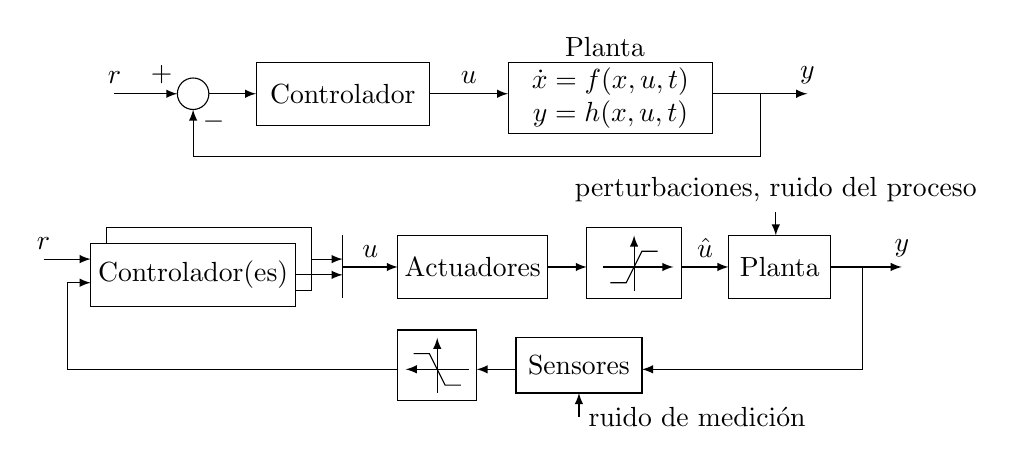
\begin{tikzpicture}
\draw (2.2,4.4) node[right]{Planta};
\draw  (1.6,4.2) rectangle (4.2,3.3) node[midway,align=center] { $\dot{x}=f(x,u,t)$\\$y=h(x,u,t)$ };
\draw [-latex] (0.6,3.8)  -- (1.6,3.8) node[above,midway]{$u$};
\draw  (-1.6,4.2) rectangle (0.6,3.4) node[midway,align=center] {Controlador};
\draw [-latex](-2.2,3.8) -- (-1.6,3.8);
\draw [-latex](-2.4,3.8) ellipse (0.2 and 0.2);
\draw [-latex](-3.4,3.8) node[above] {$r$} -- (-2.6,3.8) node[above, near end] {$+$};
\draw [-latex](4.2,3.8) -- (5.4,3.8) node[above] {$y$};
\draw [-latex](4.8,3.8) -- (4.8,3) -- (-2.4,3) -- (-2.4,3.6) node[right, near end] {$-$};


\draw  (4.4,2) rectangle (5.7,1.2) node[midway,align=center] {Planta};
\draw  (-3.7,1.9) rectangle (-1.1,1.1) node[midway,align=center] {Controlador(es)};
\draw  (2.6,2.1) rectangle (3.8,1.2);
\draw (2.9,1.4)  -- (3.1,1.4) -- (3.3,1.8) -- (3.5,1.8);
\draw [-latex](3.2,1.3) -- (3.2,2);
\draw [-latex](2.8,1.6) -- (3.7,1.6) ;
\draw (-3.5,1.9) -- (-3.5,2.1) -- (-0.9,2.1) -- (-0.9,1.3) -- (-1.1,1.3);
\draw [-latex](3.8,1.6) -- (4.4,1.6) node[above, midway]{$\hat{u}$};
\draw  (0.2,2) rectangle (2.1,1.2) node[midway,align=center] {Actuadores};
\draw [-latex](2.1,1.6) -- (2.6,1.6);
\draw [-latex](-1.1,1.5) -- (-0.5,1.5);
\draw [-latex](-0.9,1.7) -- (-0.5,1.7);
\draw (-0.5,2) -- (-0.5,1.2);
\draw [-latex](-0.5,1.6) -- (0.2,1.6) node[midway, above]{$u$};
\draw [-latex](-4.3,1.7) node[above] {$r$} -- (-3.7,1.7);
\draw  (1.7,0.7) rectangle (3.3,0) node[midway,align=center] {Sensores};
\draw [-latex](5.7,1.6) -- (6.6,1.6) node[above]{$y$};
\draw [-latex](6.1,1.6) -- (6.1,0.3) -- (3.3,0.3);
\draw [-latex](0.2,0.3) -- (-4,0.3) -- (-4,1.4) -- (-3.7,1.4);

\draw [-latex](1.1,0.3) -- (0.3,0.3);
\draw [-latex](0.7,0) -- (0.7,0.7);
\draw (1,0.1) -- (0.8,0.1) -- (0.6,0.5) -- (0.4,0.5);
\draw  (0.2,0.8) rectangle (1.2,-0.1);
\draw [-latex](1.7,0.3) -- (1.2,0.3);
\draw [-latex](2.5,-0.3) node[right]{ruido de medición} -- (2.5,0);
\draw [-latex](5,2.3) node[above]{perturbaciones, ruido del proceso}-- (5,2);

\end{tikzpicture}